%% ----------------------------------------------------------------
%% MAIN FILE (the one that you compile with LaTeX)
%% ---------------------------------------------------------------- 


% \documentclass[a4paper, 11pt, twoside, openright]{uis-thesis}
\documentclass[a4paper, 11pt]{uis-thesis}
\graphicspath{{figures/}}  % Location of the graphics files (set up for graphics to be in PDF format)

% Include any extra LaTeX packages required
\usepackage[square, numbers, comma, sort&compress]{natbib}  % Use the "Natbib" style for the references in the Bibliography
\usepackage{verbatim}  % Needed for the "comment" environment to make LaTeX comments
% \usepackage{vector}  % Allows "\bvec{}" and "\buvec{}" for "blackboard" style bold vectors in maths
\usepackage{algorithm}
\usepackage{algorithmic}
\usepackage[T1]{fontenc}
\usepackage{subfigure}
\usepackage{venturis2}
\usepackage{lmodern}
\usepackage{textcomp}    % solve issues with lmodern
\usepackage{amsfonts}
\usepackage{amsmath}
\usepackage{amsthm}
\usepackage{pdfpages}
\usepackage{microtype}   % better typesetting with pdfLaTeX
\usepackage[compact]{titlesec}
\usepackage{booktabs}
\usepackage{sectsty}     % section titles in specified font face
\usepackage{tabulary}

\allsectionsfont{\sffamily}
\numberwithin{algorithm}{chapter}
\setcounter{secnumdepth}{2}
\setcounter{tocdepth}{2}
\renewcommand{\captionlabelfont}{\sffamily\bfseries}
\newtheorem{thm}{Theorem}
\renewcommand{\algorithmicrequire}{\textbf{Input:}}
\renewcommand{\algorithmicensure}{\textbf{Output:}}
\hypersetup{urlcolor=blue, colorlinks=true}  % Colours hyperlinks in blue, but this can be distracting if there are many links.

\newcommand{\todo}[1]{\textcolor{red}{#1}}
\newcommand{\instructions}[1]{\textcolor{blue}{#1}}


\listfiles

%\usepackage[draft]{hyperref}
%\usepackage[hyperfootnotes=false,plainpages=false]{hyperref}
%% ----------------------------------------------------------------
\begin{document}
\frontmatter	  % Begin Roman style (i, ii, iii, iv...) page numbering
% Fill your name and supervisor name and sign it and replace the frontpage.
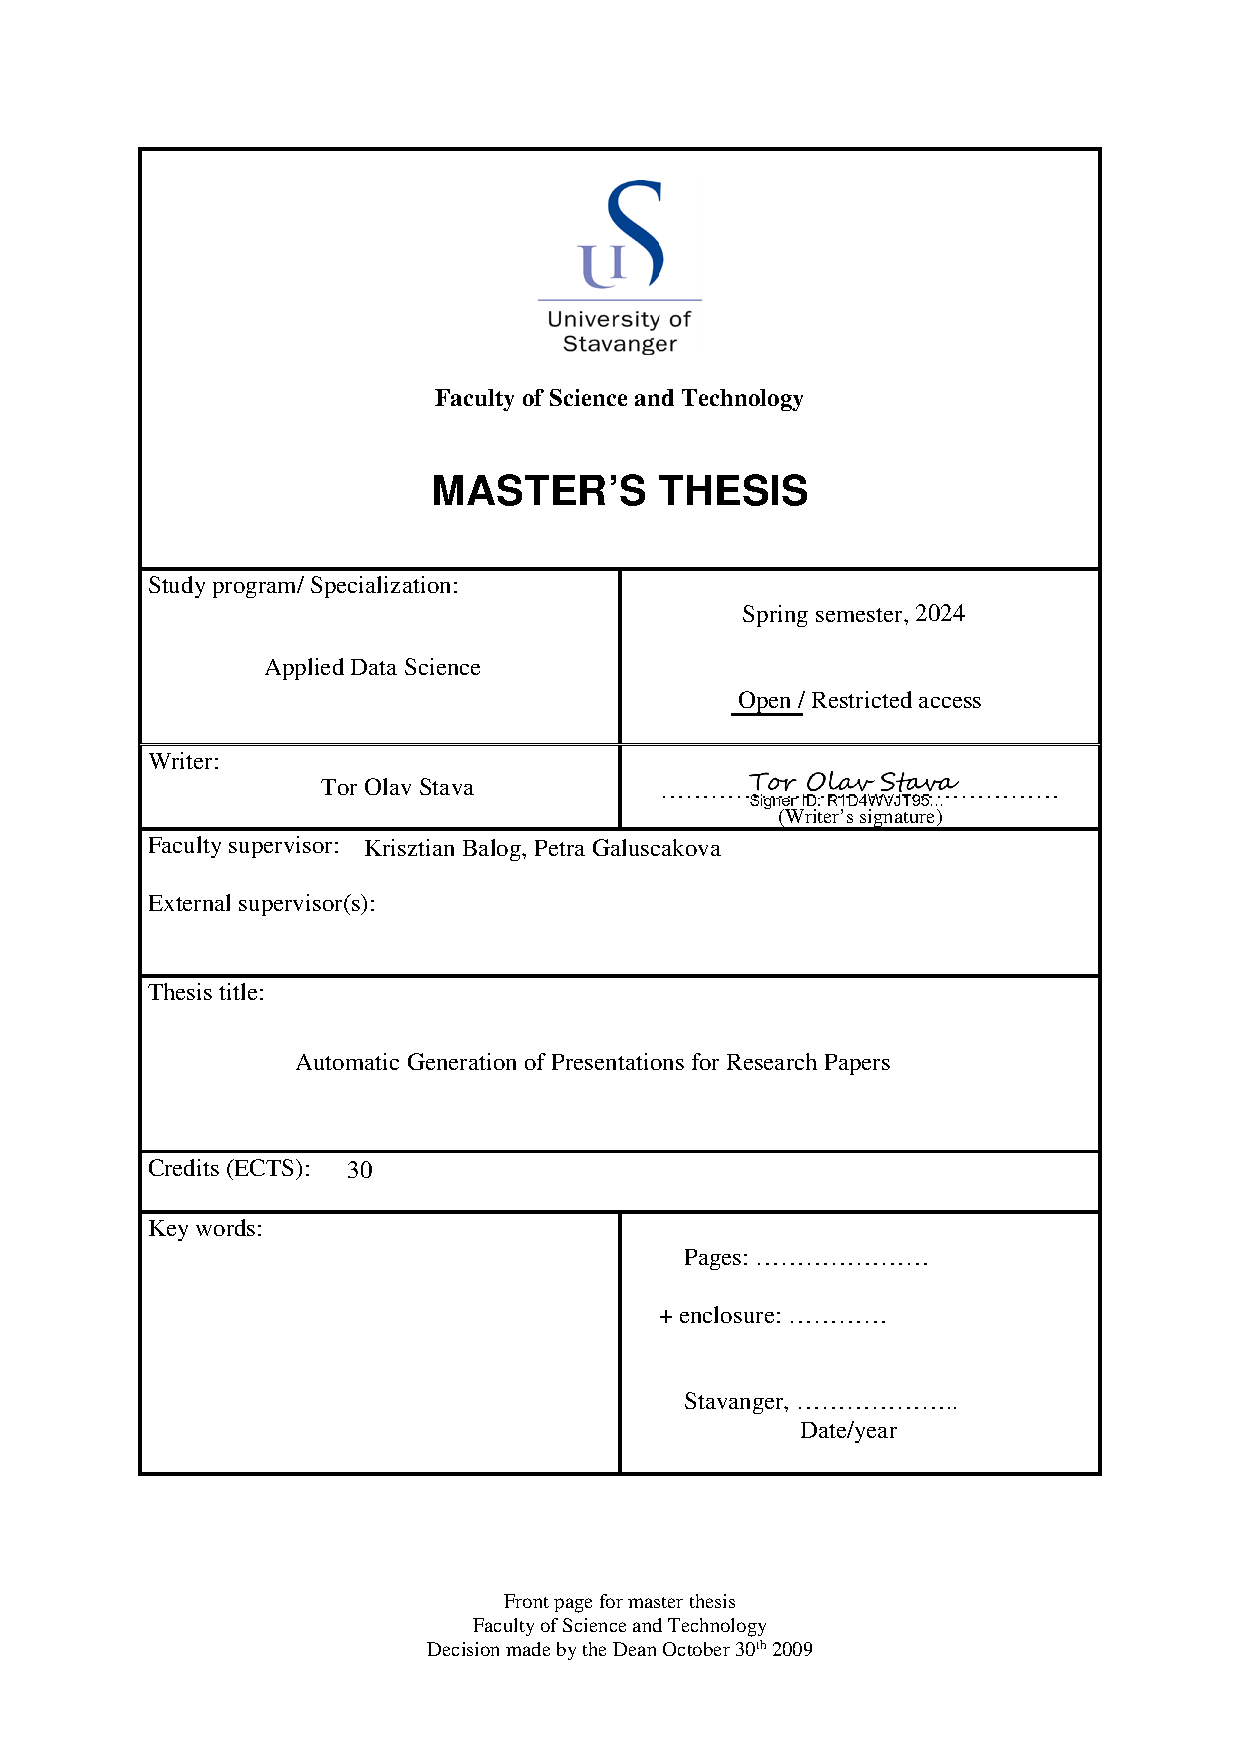
\includepdf[offset=25mm -25mm, scale=1]{./frontpage-masters-signed.pdf}


\title{Automatic Generation of Presentations for Research Papers}
\authors{Tor Olav Stava}
\addresses{\groupname\\\deptname\\\univname}  % Do not change this here, instead these must be set in the "Thesis.cls" file, please look through it instead
\date       {\today}
\subject    {}
\keywords   {}

\maketitle
%% ----------------------------------------------------------------

\setstretch{1.3}  % It is better to have smaller font and larger line spacing than the other way round

% Define the page headers using the FancyHdr package and set up for one-sided printing
%\fancyhead{}  % Clears all page headers and footers
%\rhead{\thepage}  % Sets the right side header to show the page number
%\lhead{}  % Clears the left side page header

% \pagestyle{fancy}  % Finally, use the "fancy" page style to implement the FancyHdr headers
% \fancyhead[RE,LO]{\sffamily\bfseries\nouppercase{\rightmark}}
% \fancyhead[LE,RO]{\thepage}


%% ----------------------------------------------------------------
\pagestyle{empty}  % No headers or footers for the following pages
% % % Declaration Page required for the Thesis, your institution may give you a different text to place here
% \Declaration{

% \addtocontents{toc}{\vspace{1em}}  % Add a gap in the Contents, for aesthetics

%TODO: use macro for authors; if multiple, we should say "We" instead of "I"
% I, Vinay Setty, declare that this thesis titled, `Efficiently Identifying Interesting Time Points in Text Archives' and the work presented in it are my own. I confirm that:

% \begin{itemize} 
% \item[\tiny{$\blacksquare$}] This work was done wholly or mainly while in candidature for a master's degree at this University.
  
% \item[\tiny{$\blacksquare$}] Where I have consulted the published work of others, this is always clearly attributed.
 
% \item[\tiny{$\blacksquare$}] Where I have quoted from the work of others, the source is always given. With the exception of such quotations, this thesis is entirely my own work.
 
% \item[\tiny{$\blacksquare$}] I have acknowledged all main sources of help.

% \end{itemize}
%  \vspace{5pt}
% Signed:\\
% \rule[1em]{25em}{0.5pt}  % This prints a line for the signature
 
% Date:\\
% \rule[1em]{25em}{0.5pt}  % This prints a line to write the date
% }
% \clearpage  % Declaration ended, now start a new page

% \clearpage
\null\vfill
% Now comes the "Funny Quote", written in italics
\textit{``Programming is a nice break from thinking.''}

\begin{flushright}
Leslie Lamport
\end{flushright}

\vfill\vfill\vfill\vfill\vfill\vfill\null

\clearpage
\addtotoc{Abstract}  % Add the "Abstract" page entry to the Contents
\abstract{
\addtocontents{toc}{\vspace{1em}}  % Add a gap in the Contents, for aesthetics

}

\clearpage

\setstretch{1.3}  % Reset the line-spacing to 1.3 for body text (if it has changed)

% The Acknowledgements page, for thanking everyone
\acknowledgements{
\addtocontents{toc}{\vspace{1em}}  % Add a gap in the Contents, for aesthetics
I would like to thank my supervisors for their fantastic enthusiasm and help with writing this thesis. 

}

\clearpage

\tableofcontents

\setstretch{1.3}  % Return the line spacing back to 1.3

\addtocontents{toc}{\vspace{2em}}  % Add a gap in the Contents, for aesthetics

%% ----------------------------------------------------------------
\mainmatter	  % Begin normal, numeric (1,2,3...) page numbering
\pagestyle{fancy}  % Return the page headers back to the "fancy" style

% Include the chapters of the thesis, as separate files
% Just uncomment the lines as you write the chapters


\chapter{Introduction}
\label{ch:intro}

% \instructions{Page budget for Introduction: 3-5 pages}

\section{Background and Motivation}
\label{sec:intro:background}

% \instructions{
% \begin{itemize}
%     \item Awaken the reader's interest and convince her why the theme is important.
%     \item Background information might be historical in nature, or it might refer to previous research or practical considerations.
%     \item Provide an example or use case for the problem.
%     \item It should be written on a level that it's understandable by anyone with a computer science master's degree.
%     \item It might contain a small handful of citations if it is needed to justify some main claims or assumptions, but this is not the part to detail any related work and/or compare among each other.
% \end{itemize}
% }

Converting research findings into presentations is a crucial task in academic and professional settings. However, it can be quite challenging. This process involves transforming detailed research papers into clear, engaging presentations that cater to various audiences, ranging from conference attendees to students. It demands a considerable amount of time, profound subject knowledge, and expertise in information design and storytelling skills.

The goal is to create a system that can automatically generate presentations from academic papers. This system will aim to improve efficiency and bridge the gap between detailed research and audience-friendly presentations. By automating this process, researchers and professionals will have more time and cognitive resources to focus on their primary work. Moreover, such a system will ensure that their findings reach a wider audience.

Automating the process of creating academic presentation slides involves several challenges. The system must accurately interpret the complex language used in academic papers, which are often filled with specific terminology and data. It should be able to identify the key points in a paper, understand the significance of different findings, and translate this information into visually appealing slides. Additionally, it must be able to adapt to the different conventions followed by various research fields, which have their own unique ways of presenting and arguing their findings.

To tackle the difficulties faced in academic research, significant advancements in natural language processing, information retrieval, and the use of machine learning, graph databases, and vector databases are required. By utilizing these technologies, it is possible to process and visually represent the complex content of academic papers. The development of such a system would considerably enhance the automation of knowledge dissemination, making it easier for academics and professionals to convert research papers into presentations. This, in turn, will increase the accessibility and impact of their work, providing greater opportunities for future research and collaborations.

\section{Objectives}
\label{sec:intro:objectives}

% \instructions{
% \begin{itemize}
%    \item Define the goals of your study. It might be presented as a bullet list.
%   \item Structure your goal by Research Questions (RQs). Describe each of the problems to address in your work and formulate for it a clear research question.``The problem of bla is about$\dots$, We formulate the following RQ1 Can we provide a method for bla such that bla bla''
% \end{itemize}
% }

The main objective of this thesis is to create an innovative system that can generate presentations automatically from academic research papers. Specifically, the system will convert research papers written in \LaTeX{} into presentations formatted in the \LaTeX{} Beamer framework. The purpose of this project is to make the process of sharing knowledge more efficient and accessible. To achieve this, the thesis will explore several critical research questions, each designed to address a distinct aspect of the system's development process.

\begin{itemize}
  \item \textbf{RQ1: Dataset Generation} – The first research question aims to determine whether it is possible to create a comprehensive dataset that includes research papers and their corresponding presentations, both formatted according to \LaTeX{} and Beamer specifications. This is a crucial step towards developing the proposed system, as it investigates the availability of source material needed for training and testing. The process will involve identifying potential sources for such documents, curating the dataset, and implementing strategies to ensure that it is diverse and representative.
  
  \item \textbf{RQ2: Information Extraction} – The second question deals with the methods to extract relevant information from research papers. This involves creating or using natural language processing techniques to identify and isolate important points, findings, and data within the complex structure of academic papers. The challenge here is two-fold: accurately discerning the content's significance among the academic jargon and structurally diverse formats of research papers.
  
  \item \textbf{RQ3: Information Summarization} – This question is a continuation of the previous one. It's about summarizing extracted information into a shorter form while retaining the main message. This summarization process is important when presenting research findings on slides. The research will explore the algorithms and techniques used for effective summarization, ensuring that the most important information is highlighted while maintaining the research's integrity and context.
  
  \item \textbf{RQ4: Presentation Generation} – The final question seeks to establish a methodology for converting summarized information into coherent and high-quality presentations. This includes not only the textual content but also the design and aesthetic aspects of the slides. The challenge is to automate the process of creating presentations that are not only informative but also visually appealing and engaging for the audience. This will require using design principles, information hierarchy, and customizable templates to create presentations that effectively communicate research findings.
\end{itemize}

This research aims to answer important questions that will benefit both academics and educators. It will provide a new tool to help them process and present documents automatically, which is currently a challenging task. The goal is to offer a comprehensive solution to the time-consuming process of presentation creation. By doing so, it will help enhance the accessibility and dissemination of scientific knowledge. Through rigorous investigation and development, this research will push the boundaries of what is possible in automatic document processing and presentation generation.

\section{Approach and Contributions}
\label{sec:intro:approach}

% \instructions{
% \begin{itemize}
%   \item Give a brief summary of your overall approach.
%   \item Summarize the specific contributions that you made in this thesis (e.g., a task definition, a method or model, a test collection, empirical results, analysis, etc.). It might be presented as a bullet list.
% \end{itemize}
% }

Converting a research paper into a presentation requires a complex process that may involve summarizing or extracting key elements, or a combination of both. This thesis presents a new system called TEX2BEAM, which automates the creation of presentation slides in \LaTeX{} Beamer format from research papers formatted in \LaTeX{}. The TEX2BEAM system is designed to intelligently navigate through the dense academic text of a research paper, extract relevant information, and distill it into a clear and concise presentation format.

The operational framework of TEX2BEAM is based on a set of advanced algorithms and methodologies that are designed to comprehend the intricate structure and content of academic papers. At first, the system uses natural language processing (NLP) techniques to analyze the text. It identifies and classifies various sections of the paper, such as the abstract, introduction, methodology, results, and conclusion. This step is pivotal in identifying the particular parts of the text that are most likely to contain crucial insights and findings that are relevant to a summarized presentation.

TEX2BEAM uses a combination of extractive and abstractive summarization techniques to create a presentation from a research paper. In the extractive phase, the system selects verbatim snippets that represent the main ideas and findings from the text. Then, in the abstractive phase, these ideas are rephrased and condensed into more concise statements that are tailored for slide-based presentation. This approach ensures that the presentation effectively captures the essence of the research paper while being engaging and accessible for the audience.

The TEX2BEAM system has a vital component in the form of an algorithm that organizes the summarized content into a well-structured and visually attractive presentation. This includes selecting the best sequence of slides, and generating or choosing suitable visual aids like figures, tables, and charts. Moreover, the algorithm applies design principles to improve readability and viewer engagement.

The TEX2BEAM tool will be thoroughly tested to evaluate its effectiveness and efficiency. The tests will measure its ability to accurately extract relevant information from research papers and create effective presentations. The evaluation will include metrics such as the accuracy of information extraction, the clarity and conciseness of the summarization, and the overall quality of the generated presentations. This evaluation will demonstrate the potential of TEX2BEAM as a valuable tool for academics and professionals, making the process of creating presentations easier and facilitating the sharing of research findings.


\section{Outline}
\label{sec:intro:outline}

% \instructions{
% \begin{itemize}
%     \item Give an overview of the main points and the structure of your thesis. ``Chapter 2 covers ... Chapter 3 describes ... ''
%     \item Show in a natural way how the different parts (chapters) relate to each other.
% \end{itemize}
% }

This thesis has been written to present a logical and comprehensive account of the research conducted. It covers all aspects of the research work, from reviewing related studies to providing concluding remarks on the findings and future prospects. Each chapter has been carefully crafted to build upon the previous one, taking the reader on a journey of developing the TEX2BEAM system, which is an innovative solution for generating presentations from research papers automatically.

\textbf{Chapter 2} explores the existing body of work that is relevant to the core objectives of the thesis. It delves into the methodologies and technologies that are used for summarizing texts, extracting key information, and generating presentations from academic documents and reports. The purpose of this chapter is to position the current research within the broader academic discourse by highlighting the advancements in the field and identifying the gaps that the TEX2BEAM system aims to address.

\textbf{Chapter 3} describes the methodology and technical framework used to develop the TEX2BEAM system. It explains the architectural design, algorithms, and computational strategies employed to process research papers written in \LaTeX{} format and convert them into informative and visually appealing presentations in \LaTeX{} Beamer format. The approach incorporates novel features, including the system's ability to parse academic language intelligently, identify significant content, and summarize and represent this information effectively in a presentation-ready format.

\textbf{Chapter 4} is focused on evaluating the performance of the TEX2BEAM system. It presents a detailed analysis of the system's accuracy in extracting information, effectiveness in summarizing content, and the overall quality and coherence of the generated presentations. The evaluation process includes both quantitative measures and qualitative feedback, providing a comprehensive understanding of the system's capabilities, limitations, and potential impact on the field.

\textbf{Chapter 5} concludes the thesis and provides a summary of the key insights and contributions made through the research. It highlights the significance of automating the process of generating presentations from research papers and discusses the implications for academic and professional dissemination of knowledge. Furthermore, this chapter outlines potential areas for future research, proposing ways in which the TEX2BEAM system could be improved, expanded, or used in new areas.


\chapter{Related Work}
\label{ch:related}

% \instructions{Page budget for Related Work: 10 - 15 pages
% \begin{itemize}
%     \item Discuss the relevant literature related with your problem, in a coherent way to demonstrate that you have given due consideration to know: your problem and the possible sub-problems of interest in this work, the previous approaches, and their benefits and missing points or drawbacks.
%     \item It is not about concatenating summaries of papers. Rather, it is about to discuss the problem, its details and challenges (difficulties and/or opportunities) you focus on, all this by relying on previous work, comparing what some did, what some else improved or added, what is missing, and so on.
%     \item Moreover, mind to keep the focus in the areas you care during your discussion (since you control the story), and to remark what you consider useful, interesting, or challenging.
%     \item In some cases it could be necessary and/or natural to have, first, an introduction (which could discuss works on more general aspects of the problem), and then split the rest of the chapter in sections, each discussing a particular aspect of the problem.
%     \item If you define a new task, or create or improve a method, or develop a test collection, or perform a missing major evaluation, explain why it is interesting, why is different or helpful versus previous works.
%     \item Mind that the reader may have never heard about these things. You need to discuss them in such detail that it is possible to follow later parts of the thesis without having to consult external resources.
%     \item Always use natbib!
%     \item Use \texttt{\textbackslash\.citet\{\}} for textual citation. For example, ``\citet{Balog:2018:Book} proposed...''
%     \item Use \texttt{\textbackslash\.citep\{\}} for parenthetical citation. For example, ``In \citep{Zhang:2020:KDD} the idea of ..''
%     \item Here is an example of a PhD thesis:  \citet{Maxwell:2019:PhDThesis} 
%     \item Here is how a Journal article would look in the Bibliography: \citet{Sanderson:2010:FnTIR}
%     \item Never write out Smith et al., there is a \texttt{\textbackslash\.citeauthor{}\{\}} command for that (but most likely what you're looking for is actually \texttt{\textbackslash\.citet\{\}}.
%     \item Check the corresponding Bib entry, for citing online documentation~\citep{Rasa:2022:doc}; if you just need to include an URL of a website/code/dataset, use a footnote instead.\footnote{\url{https://rasa.com}}
% \end{itemize}
% }

\textbf{Automatic slide generation of scientific papers}\citep{Sefid:2019:K-CAP}

\textbf{ArXiv Table Extractor}\citep{Ramsay:2021:BachelorThesis}

\textbf{DOC2PPT: Automatic Presentation Slides Generation from Scientific Documents}\citep{Fu:2022:AAAI}

\textbf{PDF2LaTeX: A Deep Learning System to Convert Mathematical Documents from PDF to LaTeX}\citep{Wang:2020:DocEng}\footnote{\url{https://github.com/senyalin/PDF2LaTeX}}\footnote{\url{https://github.com/wzlxjtu/PDF2LaTeX-dataset}}
\chapter{Approach}
\label{ch:approach}

\instructions{Page budget for Approach: 20-30 pages
%
\begin{itemize}
    \item This chapter describes your main contributions (i.e., what you did) and the decisions that went into them (i.e., why did you did it the way you did it).
    \item Alternative headings may be used depending on the kind of contribution(s) you make.
\end{itemize}
}

\section{Overview}

\instructions{
\begin{itemize}
    \item This section should explain the high-level design
    \item Include possibly an architecture figure that shows how the different parts fit together and what processing/technology/tools/datasets have been used for the different components.
\end{itemize}
%
Name these themes based on the different components or sub-problems you are solving in your thesis.
}
    
\section{Theme 1}
\section{Theme 2}

\instructions{
\begin{itemize}
    \item For larger/more complex projects, the separate themes may be chapters on their own (e.g., components in a system; sub-problems of a major evaluation study; etc.).
    \item Include screenshots, examples, tables, algorithms (with pseudo code), plots for some preliminary observations leading to some aspect of your approach decisions, etc. so that it's not just text.
    \item Always discuss the alternatives considered and the rationale for the choosing the solutions you adopted.
\end{itemize}
}

\chapter{Experimental Evaluation}
\label{ch:eval}

\instructions{
Page budget for Evaluation: 10-15 pages
%
\begin{itemize}
    \item Detail your evaluation methodology, present your results, and provide an analysis of them. Results can be quantitative and/or qualitative (from benchmark, user study, user satisfaction survey, etc.).
    \item It is strongly desired that you have empirical results, nevertheless, this may not be applicable to all types of theses.
\end{itemize}
}

\section{Experimental Setup}
\label{sec:eval:expsetup}

\instructions{
\begin{itemize}
    \item Explain the methodology used for evaluating your contribution, and the metrics used for evaluation.
    \item If you use any dataset, explain it, detail its version, and mention briefly some main statistics about it, of interest for your problem (e.g., size, provenience, etc.), if appropriate.
    \item If you collect ground truth data, describe your annotation experiment. Explain what the annotators were asked to do (and show a screenshot or schema if available). Detail the number of annotators, their nature (experts, or crowdworkers), the criteria for deciding on each annotation instance (e.g., majority class, dynamic judgments, etc.), the criteria for ensuring quality (e.g., minimum accuracy, filters). If possible, report the inter-annotator agreement coefficient and mention how strong this value means that the agreement is.
\end{itemize}
}

\section{Experimental Results}
\label{sec:eval:results}


\instructions{
\begin{itemize}
    \item Present the results, using tables and (pretty) plots.
\end{itemize}
}

\section{Analysis}
\label{sec:eval:analysis}

\instructions{
\begin{itemize}
    \item Now that you presented the results, what do these results actually mean (esp. regarding the objectives you set out in the introduction)? 
    \item Can you identify success and failure cases? 
    \item What do the results say for individual parts you evaluate and overall in combination? 
    \item Make sure you formulate clear take-home messages.
\end{itemize}
}

\chapter{Conclusions}
\label{ch:conclusion}

\instructions{Page budget for Conclusions: 3-5 pages
%
\begin{itemize}
    \item Summary of the work you have done, what worked and what didn't
    \item Make sure it connects well with the Introduction, by answering every RQ.
\end{itemize}
}

\section{Future Directions}
\label{sec:conclusions:future}

\instructions{Discuss potential future work that may fill gaps in your work, or approaches that seem promising to overcome problems you encountered but that you weren't able to tackle.}


%% ----------------------------------------------------------------
% Now begin the Appendices, including them as separate files

% \addtocontents{toc}{\vspace{2em}} % Add a gap in the Contents, for aesthetics

% \appendix % Cue to tell LaTeX that the following 'chapters' are Appendices
% \chapter{Sample Appendix Contents}

\instructions{
The following may (optionally) go to an appendix chapter:
%
\begin{itemize}
    \item More detailed evaluation results.
    \item Longer details on a possible annotation experiment.
    \item Hyperparameter tuning and detailed experimental setup.
    \item Setup and installation instructions to repeat the experiments etc.
\end{itemize}
}
% \chapter{Instructions to Compile and Run System}
\label{apx:instructions}

\instructions{
This appendix may contain following:
%
\begin{itemize}
    \item Installation instructions
    \item Source code / class structure
    \item More detailed evaluation results
\end{itemize}
}


% \addtocontents{toc}{\vspace{2em}}  % Add a gap in the Contents, for aesthetics
\backmatter

%% ----------------------------------------------------------------
\label{Bibliography}
\lhead{\emph{Bibliography}}  % Change the left side page header to "Bibliography"
\bibliographystyle{unsrtnat}  % Use the "unsrtnat" BibTeX style for formatting the Bibliography
\bibliography{Bibliography}  % The references (bibliography) information are stored in the file named "Bibliography.bib"

\end{document}
